\documentclass{beamer}
%\usetheme{Boadilla}
%\usetheme{Darmstadt}
%\usetheme{Berkeley}
%\usetheme{Berlin}
%\usetheme{Copenhagen}
\usetheme{Warsaw}

\DeclareMathOperator*{\argmax}{arg\,max} % Jan Hlavacek

\title{Developing Strategies with Reinforcement Learning}
\subtitle{FCOS Short Version}
\author{Cdt Koen Boeckx, Ir}
\date{April 27, 2020}

\begin{document}

\begin{frame}
\titlepage
\end{frame}

\begin{frame}{Outline}
\tableofcontents
\end{frame}

\section{Introduction}
\begin{frame}
\frametitle{Introduction}
\begin{itemize}
    \item What is Multi-Agent (MA) learning
    \item What is Reinforcement Learning (RL)?
    \item How do we combine both?
    \item What am I working on?
    \item Where can you work on?
\end{itemize}
\end{frame}

\begin{frame}
\frametitle{The IRIS Project}
\begin{block}{Intelligent Recognition Information System}
\begin{itemize}
    \item Piloted by \emph{John Cockerill Defence}
    \item Funding provided by Walloon governement
    \item Goal: develop a pipeline from observation to action suggestion on board of armoured vehicles
    %\item I've worked on strategy development
\end{itemize}
\end{block}
\begin{figure}[htp]
    \centering
    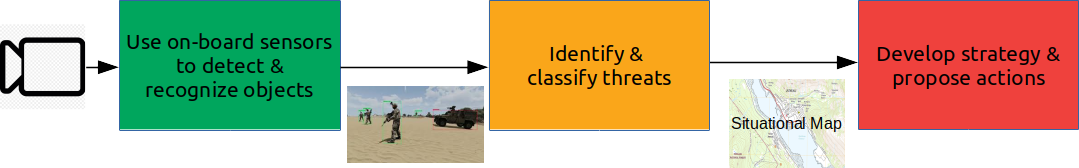
\includegraphics[width=11cm]{images/IRIS_schematic.png}
\end{figure}
\end{frame}

\begin{frame}
\frametitle{Goals of my thesis}
\begin{block}{1. Battlefield Modelling}
\begin{itemize}
    \item An algorithm that simulates a real environment
    \item Simple enough to use
    \item Realistic enough to be useful
\end{itemize}
\end{block}
\pause
\begin{block}{2. Develop strategies}
\begin{itemize}
    \item Use \emph{Reinforcement Learning} to develop strategies
    \item Assess performance of different RL algorithms
\end{itemize}
\end{block}
\end{frame}

\section{Reinforcement Learning}
\begin{frame}
\frametitle{Reinforcement Learning}
\begin{columns}
\column{0.5\textwidth}
\begin{alertblock}{Reinforcement Learning}
\begin{itemize}
    \item Learn a policy $\pi$ through interaction with environment
    \item No explicit examples, just a reward signal
\end{itemize}

\end{alertblock}
\begin{figure}[htp]
    \centering
    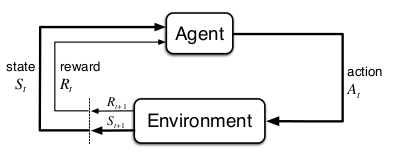
\includegraphics[scale=0.4]{images/mdp.png}
\end{figure}
\column{0.5\textwidth}
\begin{block}{Markov Decision Process}
\begin{itemize}
    \item Agent takes actions based on state
    \item Based on action, the environment changes state and returns reward
    \item Goal: maximize cumulative reward $G_t$
    \begin{equation*}
        G_t &= \sum_{k=0}^{\infty} \gamma^k R_{t+k+1}
    \end{equation*}
    \item Discount factor $\gamma$
\end{itemize}
\end{block}
\end{columns}
\end{frame}

\begin{frame}
\frametitle{Reinforcement Learning}
\begin{block}{Value approximation}
\begin{itemize}
    \item Estimate the value $Q(s,a) $ of taking action $a$ in state $s$
    \item Derive a policy from this estimated value: $\pi_{*}(s) = \argmax_{a} Q(s, a)$
    \item \emph{Q-learning}: derive $Q(s,a)$ with Bellman equation
\end{itemize}
\end{block}

\begin{block}{Policy approximation}
\begin{itemize}
    \item Learn the optimal policy $\pi_{*}$ directly
    \item Update the policy parameters with the \emph{policy gradient theorem}
    \item $\bm{\theta}_{t+1} = \bm{\theta}_t + \alpha \, G_t \, \frac{\nabla_{\bm{\theta}_t} \pi(A_t|S_t, \bm{\theta}_t)}{\pi(A_t|S_t, \bm{\theta}_t)}$
\end{itemize}
\end{block}
\end{frame}

\begin{frame}
\frametitle{Deep Reinforcement Learning}
\begin{itemize}
    \item Classical RL algorithms work with tables that store $Q$-values or policies
    \item This is no longer feasible when the state space becomes large
    \pause
    \item Solution: work with function approximators $f(s; \theta)$
    \item \emph{Deep Learning}: artificial neural networks as function approximators
\end{itemize}
\end{frame}

\begin{frame}
\frametitle{Deep Learning}
\begin{columns}
\column{0.5\textwidth}
\begin{figure}[htp]
    \centering
    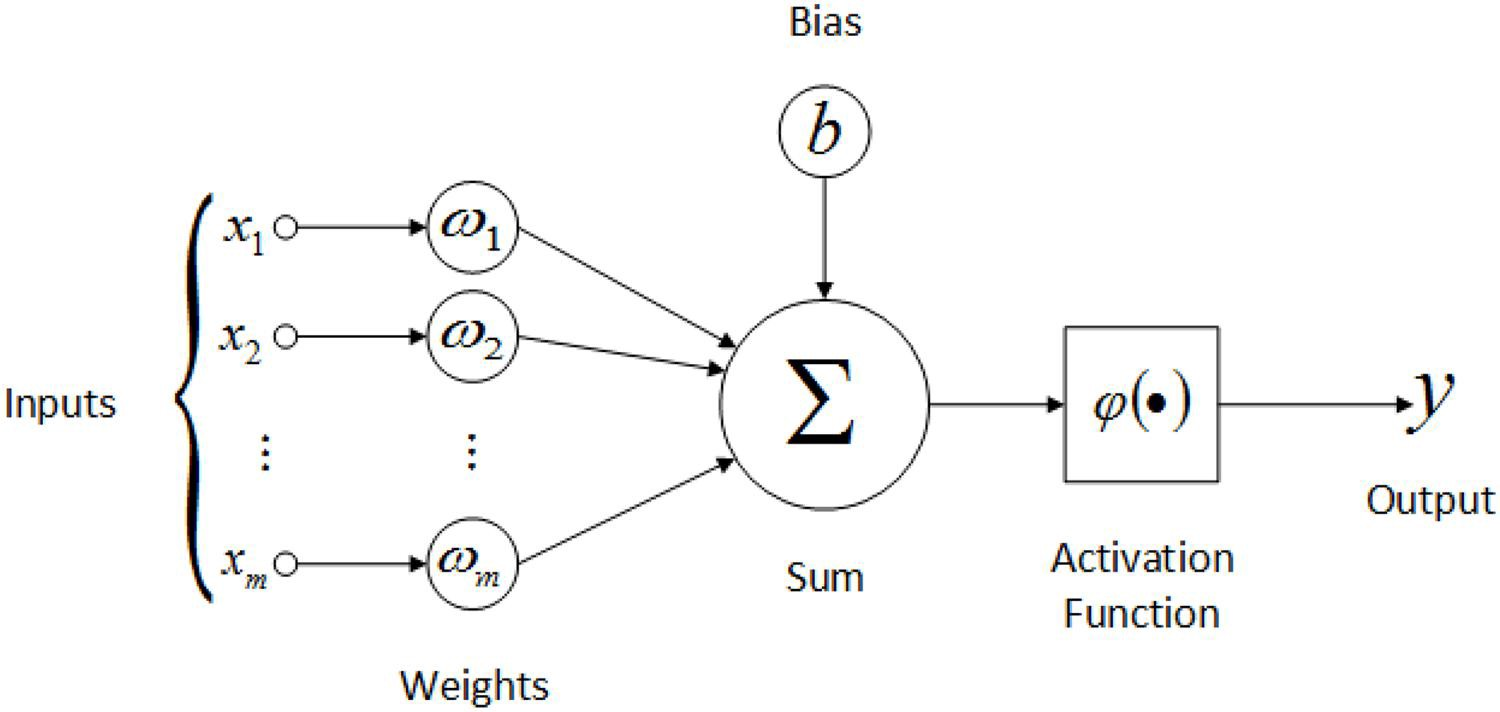
\includegraphics[scale=0.1]{images/neuron.jpeg}
    \caption{A Neuron}
\end{figure}
\column{0.5\textwidth}
\begin{figure}[htp]
    \centering
    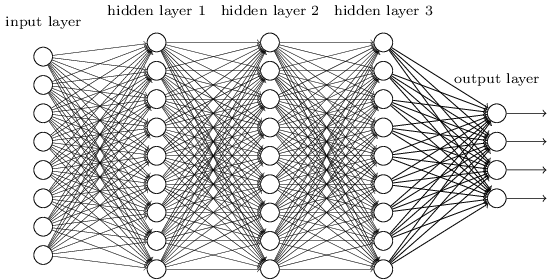
\includegraphics[scale=0.3]{images/neural_net.png}
    \caption{A Neural Net}
\end{figure}
\end{columns}
\end{frame}

\begin{frame}
\frametitle{Deep Reinforcement Learning}
\begin{block}{Deep Q-networks}
\begin{itemize}
    \item Use a neural net to estimate the value of a state $S$
    \item Loss function $\mathcal{L} = \big [R_t + \gamma \max_{A'} Q(S_{t+1}, A';\, \bm{\theta}) - Q(S_t, A_t); \theta \big ]^2$
\end{itemize}
\end{block}
\begin{block}{Deep Policy Gradients}
\begin{itemize}
    \item Use a neural net to represent a policy
\end{itemize}
\begin{figure}[htp]
    \centering
    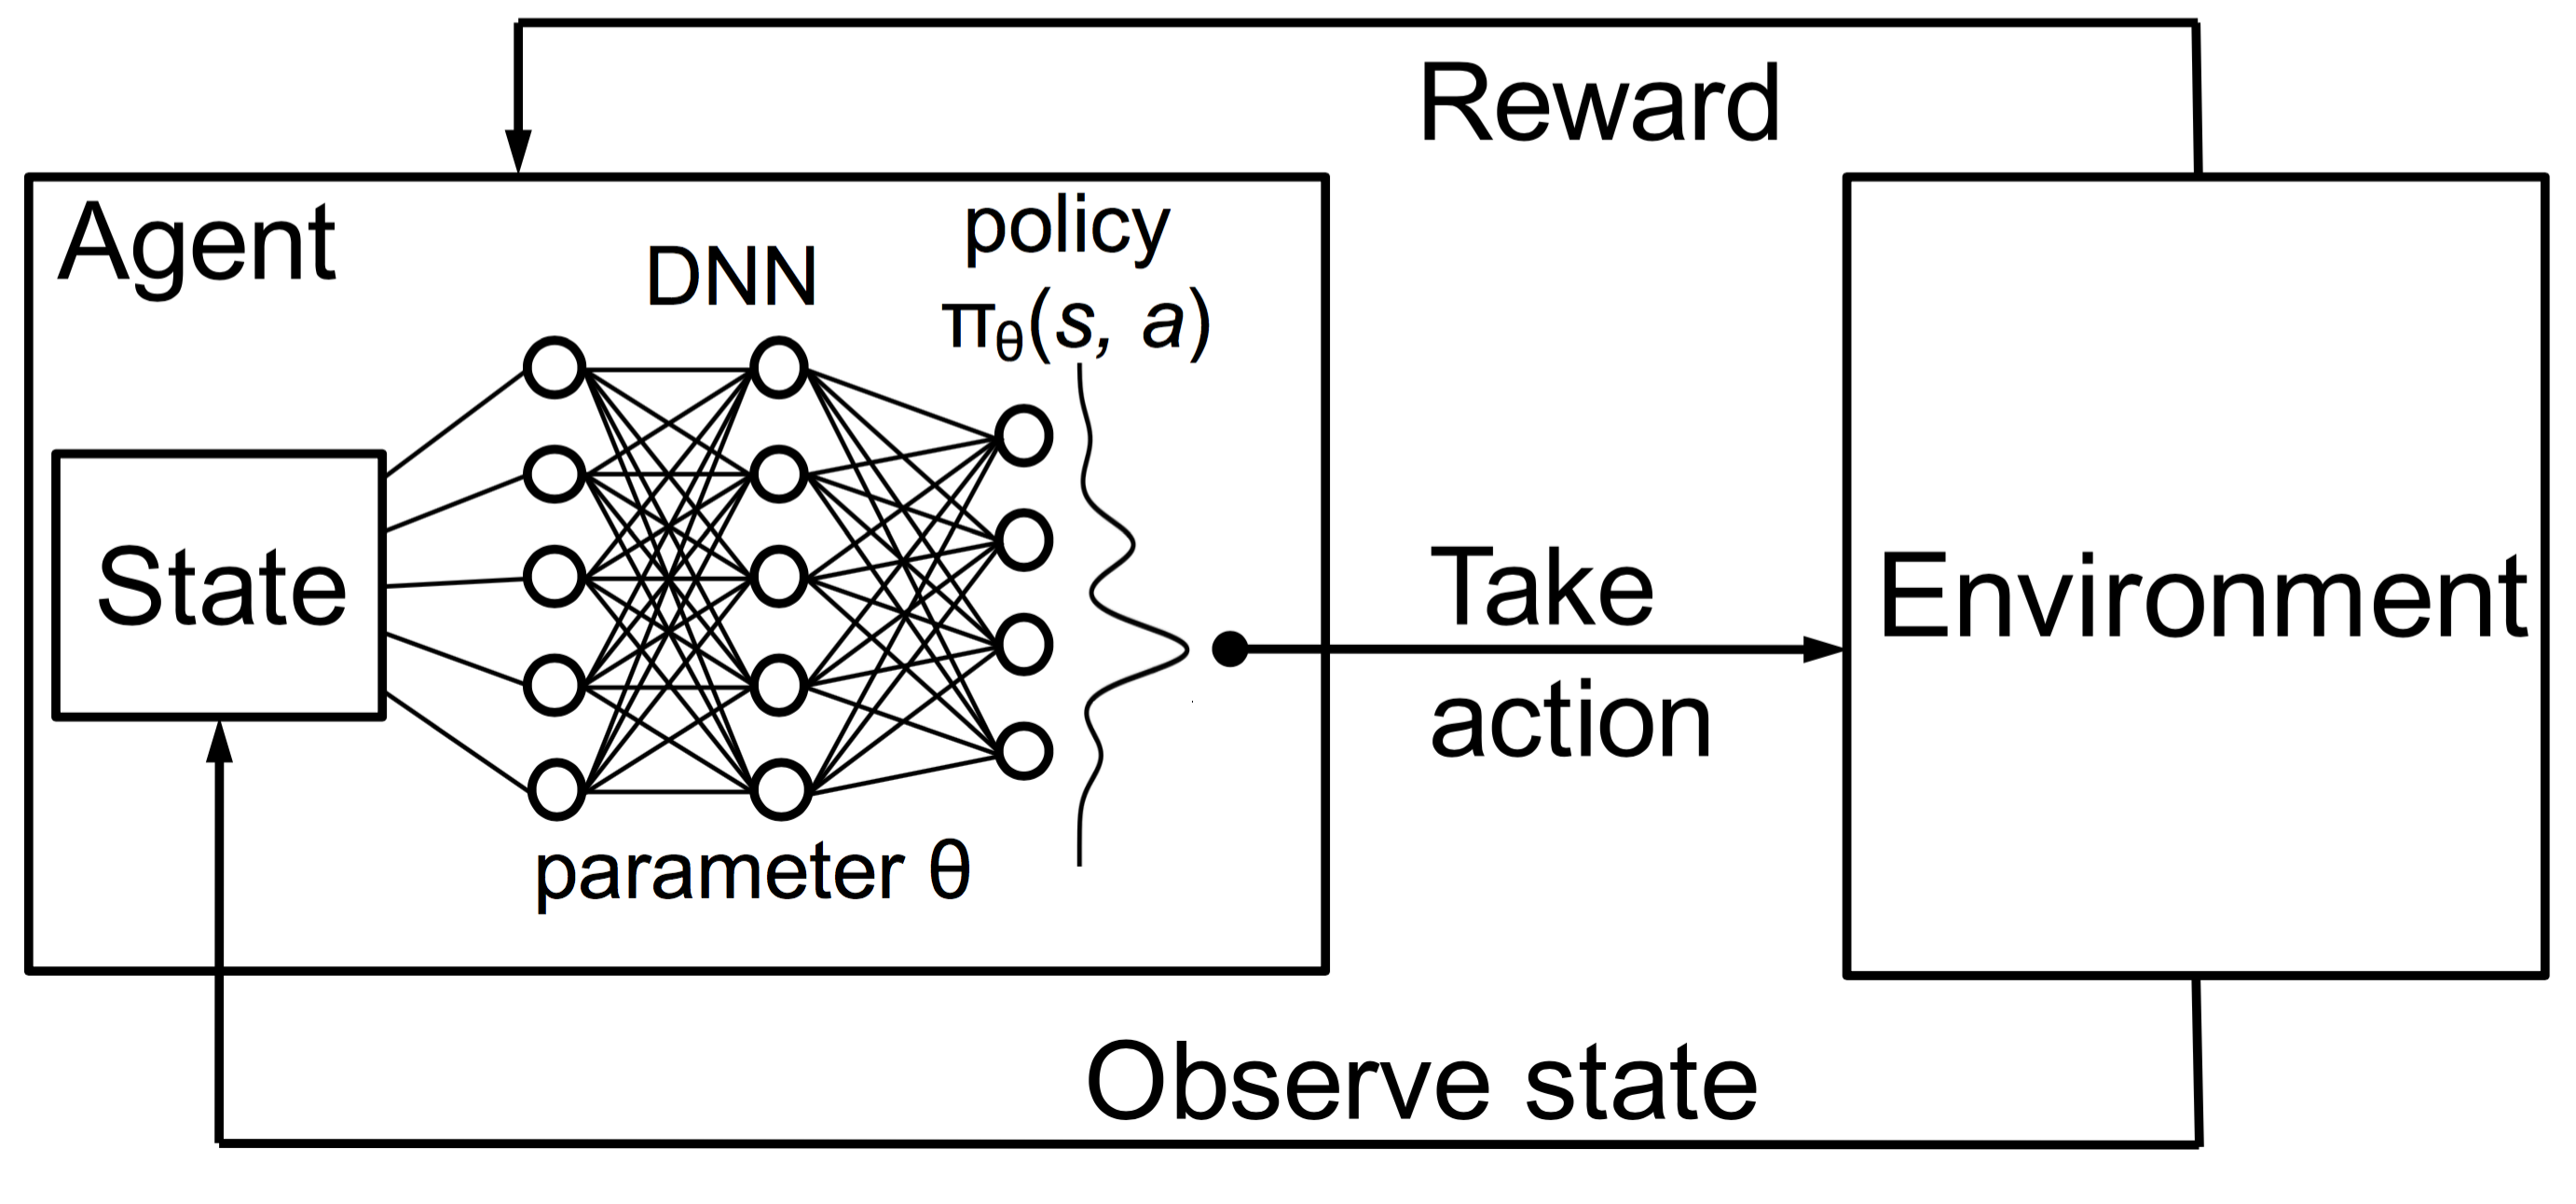
\includegraphics[width=6cm]{images/deep_pg.png}
\end{figure}
\end{block}
\end{frame}

\begin{frame}
\frametitle{Multi-Agent Learning}
\begin{itemize}
    \item Extension of MDP framework
    \item Multiple adaptive agents are present
    \item The agents receive a single reward, based on their joint action set
    \item Allows for emergent strategies, but difficult to train
    \item \emph{Credit assignment}: which agent deserves the credit for the win
\end{itemize}
\end{frame}

\begin{frame}
\frametitle{Multi-Agent Learning Algorithms}
\begin{block}{Independent Agents}
\begin{itemize}
    \item Just assumes all agents are independent
    \item Use single-agent algorithm for each agent
    \item $+$ : simple extension of single-agent RL
    \item $-$ : no cooperation between agents
    \item IQL, IAC
\end{itemize}
\end{block}
\begin{block}{QMix}
\begin{itemize}
    \item True multi-agent algorithm
    \item Centralised learning - Decentralised execution
    \item Compute $Q_{tot} = f(Q_1, \dots Q_N)$ such that $\frac{\partial Q_{tot}}{\partial Q_i} \geq 0$
\end{itemize}
\end{block}
\end{frame}

\begin{frame}
\frametitle{QMix}
\begin{block}{QMix}
\begin{itemize}
    \item True multi-agent algorithm
    \item Centralised learning - Decentralised execution
    \item Compute $Q_{tot} = f(Q_1, \dots Q_N)$ such that $\frac{\partial Q_{tot}}{\partial Q_i} \geq 0$
\end{itemize}
\end{block}
\begin{figure}[htp]
    \centering
    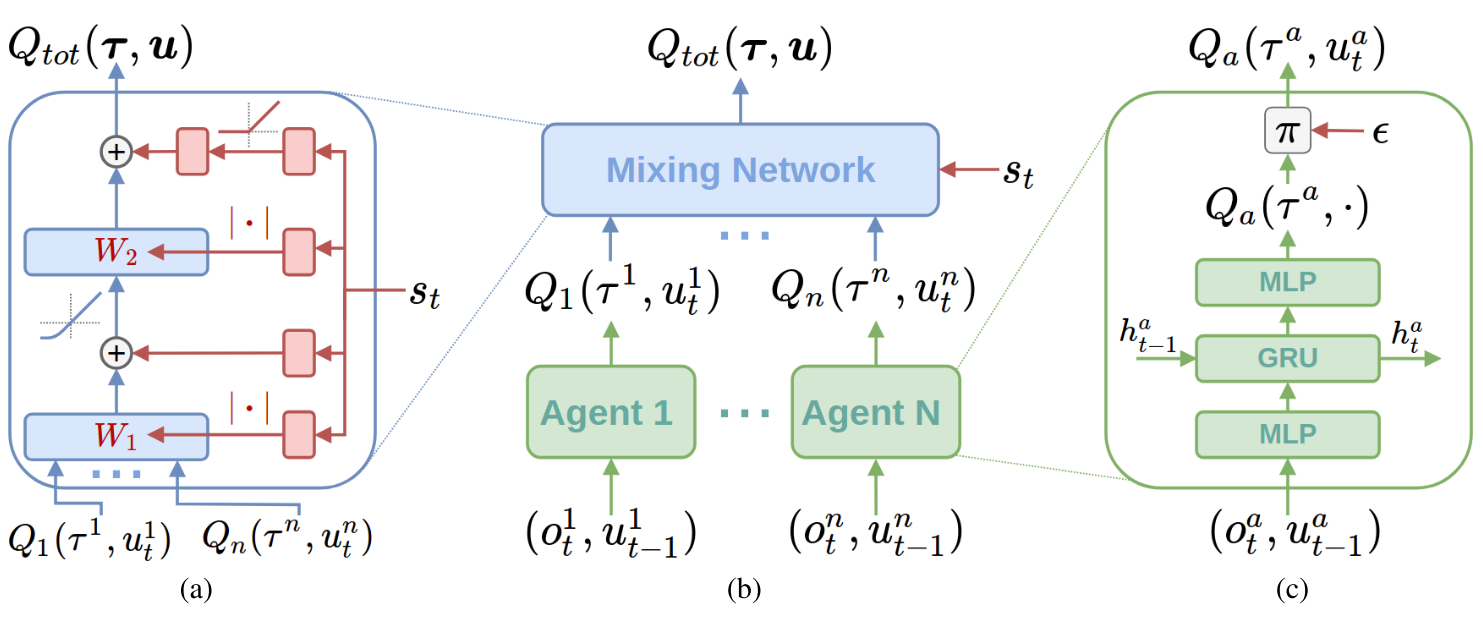
\includegraphics[scale=0.2]{images/qmix_structure.png}
\end{figure}
\end{frame}

\section{Modelling the battlefield}
\begin{frame}
...
\end{frame}

\end{document}